%\section{Problem Formulation}

\section{Correlation-based Differential Encoding}
\label{sec::DifferentialEncoding}

\begin{figure}
\begin{center}
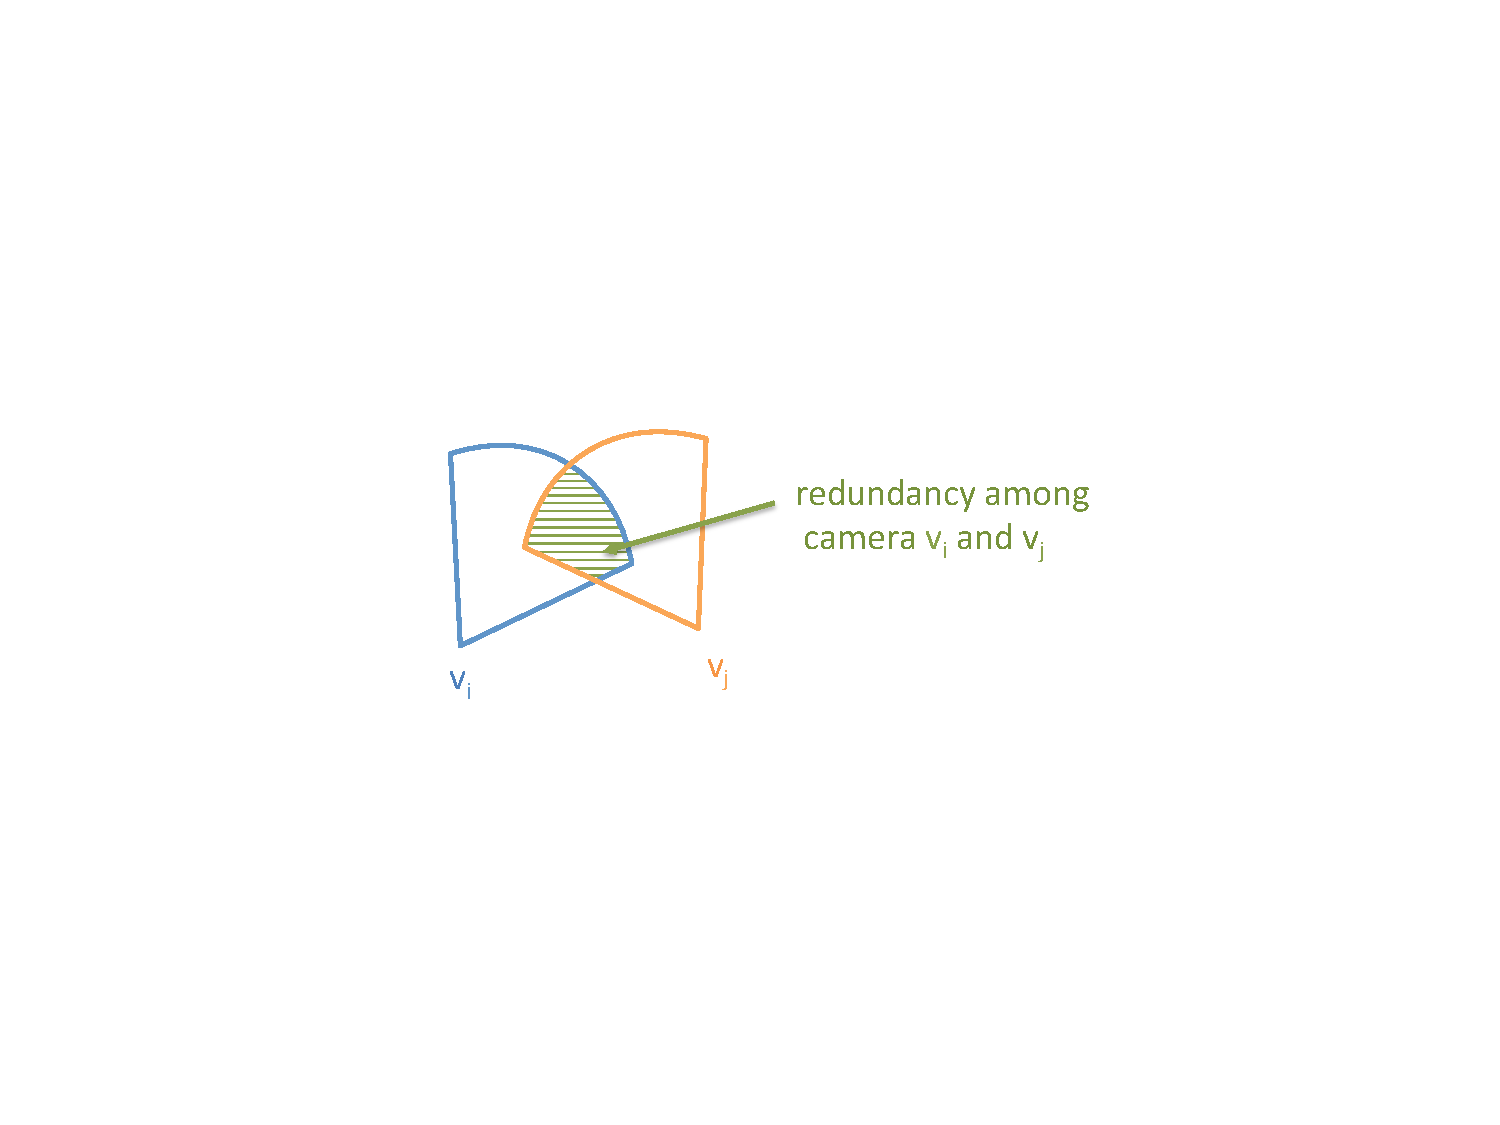
\includegraphics[width=0.7 \columnwidth]{./fig/cameraRedundancy.pdf}
\caption{\label{fig::cameraRedundancy}Redundancy among cameras}
\end{center}
\end{figure}
As we mentioned before, our purpose in this paper is to minimize the total
encoded bits for transmission of a wireless multimedia sensor network.
Given a set ${V=\{v_1,v_2, \cdots v_N \}}$ of cameras placed in a wireless
multimedia sensor network, where each camera $v_i$ produces image $X_i$.
If these cameras are deployed under a dense scenario, there might be some
redundancy among the cameras in $V$.
As Figure~\ref{fig::cameraRedundancy} shows, if two camera $v_i$ and $v_j$ are
installed at a neighboring position and both have the same area of interest,
there might have some overlap among their collected scene.
Therefore, if we serve the network in an independent way (all cameras in $V$
encode its data independently), we might cause a waste of using the limited
radio resource since there is no need to transmit the redundant part.

Since we have mentioned that using a dependent encoding scheme is a more
efficient way to serve the wireless multimedia sensor network.
It rise a problem that how to reduce the transmission of the redundant part.
For the scenario in Figure~\ref{fig::cameraRedundancy}, we can either
compress image $X_i$ based on the prediction of $X_j$ or compress $X_j$ based
on the prediction of $X_i$.
Which mode to choose should depend on the scheduling sequence of cameras, since
a camera can only compress its data based on those previous scheduled cameras.
Therefore, in order to reduce the total required encoded bits of a network, we
will explore an algorithm to determine a proper schedule in the following
sections. 